\documentclass[11]{article}
\usepackage{graphicx}
\graphicspath{ {images/} }


\title{CS2006 Haskell Project 2 - \\ Gomoku}
\date{27/04/2018}
\author{Matriculation Numbers: 160001362, 160016245, 160021429 (Group 14)}

\begin{document}
	\maketitle
	\newpage
	\tableofcontents
	
	\newpage
	\section{Summary of Functionality}
		This practical specified the development of the board game Gomoku using the functional programming language Haskell. \\\\The provided README file gives a detailed description of what the solution can do and instructions explaining how to configure settings through the command line as well as in game.
\\\\The following functionality has been implemented:
	\subsection{Basic Specification:}
		All requirements from the basic specification have been implemented. They are as follows:	
		\begin{enumerate}
			\item \textbf{Implement the game mechanics in Board.hs} -
			\item \textbf{Implement the drawWorld function in Draw.hs to display the current board state graphically} -
			\item \textbf{Implement appropriate event handlers for inputs events} -
			\item \textbf{Implement a move generator (in AI.hs) and an evaluation function (in Board.hs) to provide a computer opponent} - two AIs have been implemented, a random AI and a heuristic based AI. The random AI generates a random index refer to an element in a list of empty positions of the board and places a piece there. The heuristic AI uses the evaluation function in Board.hs to calculate its board score relative to its opponent for each possible move and chooses the highest scoring move.
		\end{enumerate}
	
	\subsection{Additional Requirements:}
	 From the suggested additional requirements, all of the easy and medium requirements have been implemented, as have the listed hard requirements:
	 	\subsubsection{Easy}
			\begin{itemize}
				\item \textbf{Easy Requirement 1} - 
				\item \textbf{Easy Requirement 2} - 
				\item \textbf{Easy Requirement 3} - 
			\end{itemize}

		\subsubsection{Medium}
			\begin{itemize}
				\item \textbf{Medium Requirement 1} - 
				\item \textbf{Medium Requirement 2} - 
				\item \textbf{Medium Requirement 3} - 
				\item \textbf{Medium Requirement 4} -
			\end{itemize}
		\subsubsection{Hard}
				\begin{itemize}
					\item \textbf{Hard Requirement 2} - 
				\end{itemize}
	\subsection{Further Features:}
		The following additional features have also been implemented:
		\begin{itemize}
			\item An iterator class, IteratorOfTwistedIntMatrix, has been implemented in twisted\_int\_matrix.py file which iterates over an instance of TwistedIntMatrix from top left to bottom right across the TwistedInt elements. As with the IteratorOfTwistedIntegers iterator, this iterator has a hasNext(), next() and \_\_init\_\_ functions.
		\end{itemize}

	\section{Design and Implementation}
		\begin{itemize}
			\item \textbf{Basic Specification - TwistedInt Data Structure (twisted\_int.py)} - 
			
			\item \textbf{Easy Requirements 1 and 2 (checker.py)} - 
			
			\item \textbf{Easy Requirement 3 (twisted\_integers.py)} - 
			
		\item \textbf{Medium Requirement 1 (twisted\_integer.py)} - 
		
		\item \textbf{Medium Requirement 2 and 3 (twisted\_integers.py)} - 
		
		\item \textbf{Hard Requirement 1 (twisted\_int\_matrix.py)} - 
		
		\item \textbf{Hard Requirement 2} - 	
		\end{itemize}
		
	\section{Evidence of Testing}	
		The code contains basic example docTests for every function. The output of which follows on the next page \footnote{Terminal output would have been directly included within this report rather than as a screen shot but the characters disagree with latex formatting}. The output of unit tests would have been displayed but as discussed in the Known Problems section, we could unfortunately not integrate them with the final implemenation. The results shown can also be found in results.txt. 
		\newpage
		
			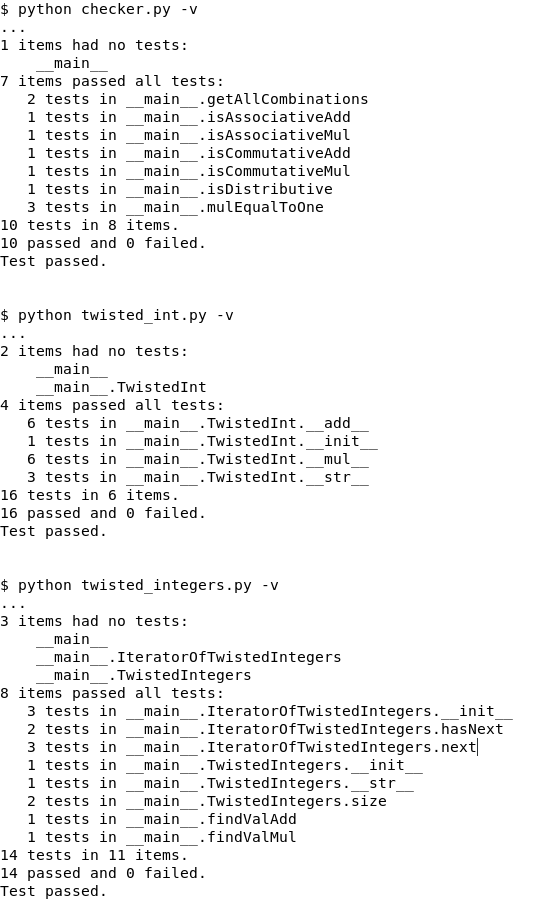
\includegraphics[scale=0.5]{Test1.png} \\\\
			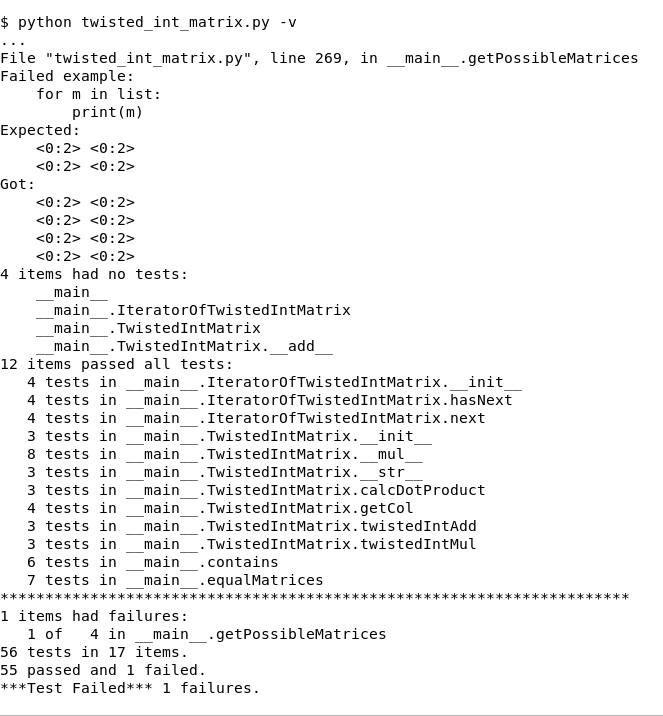
\includegraphics[scale=0.5]{Test2.png} \footnote{The 1 failure is the due to repeated results being printed due to a bug with the contains function when passing in the same matrix multiple times. This is discussed in the Known Problems section.}
		
	\section{Known Problems}
		
		
	\section{Problems Overcome}
	

	\section{Summary of Provenance}
			\begin{itemize}
				\item 160001362:
					\begin{itemize}
						\item Basic Requirement 4
						\item Hard Requirement 2 - Implemented the multiple AIs
					\end{itemize}
					
				\item 160016245:
					\begin{itemize}
						\item Easy 3 - Rule of four and four
						\item Medium 1
					\end{itemize}
					
				\item 160021429:
					\begin{itemize}
						\item Unit Testing 
					\end{itemize}
			\end{itemize}
				
	
\section{Conclusion}
In conclusion we have successfully implemented all of the basic specification, easy, medium and hard requirements without major faults. Overall this practical felt a lot more accessible than the previous practical due to the use of Python rather than Haskell. Given more time we would address the issue relating to the running of the unit tests and perhaps add more mathematical functions to the solution.

\end{document}